\documentclass{article}

\usepackage{float}
\usepackage{graphicx}
\usepackage{caption}
\usepackage{subcaption}
\usepackage{amsmath}
\usepackage[margin=0.5in]{geometry}
\title{Comparative Repeat Family Annotation with Cactus}

\begin{document}
\maketitle
\section{Detecting Candidate Repeat Insertions}


The output of a Cactus alignment is represented as a genome history graph (Fig. \ref{fig:ghg}), stored in HAL format. At each internal node in the species tree, each genome is represented by a series of segments, each of which may have a homologous segment in the parent genome. An event in the genome history graph where a segment in the parent genome has two descendants in a child genome is called a duplication. A segement that is reversed in the child genome relative to its parent is called an inversion. And a segment present in a child genome but not the parent is an insertion.

Since Cactus alignments are typically created with repeat-masked genomes, we expect most transpable element (TE) duplication events to be represented as insertions relative to the parent. Figure \ref{fig:insertion_length_dist} shows the normalized length distributions for insertions in each genome of a ten-way Cactus alignment, after filtering insertions with high N content. On the human branch, a peak is visible at $300 bp$, likely corresponding to the Alu family of retrotransposons. Figure \ref{fig:number_of_insertions} shows the total number of insertions on each branch of the ten-way alignment.
\begin{figure}[h]
  \centering
  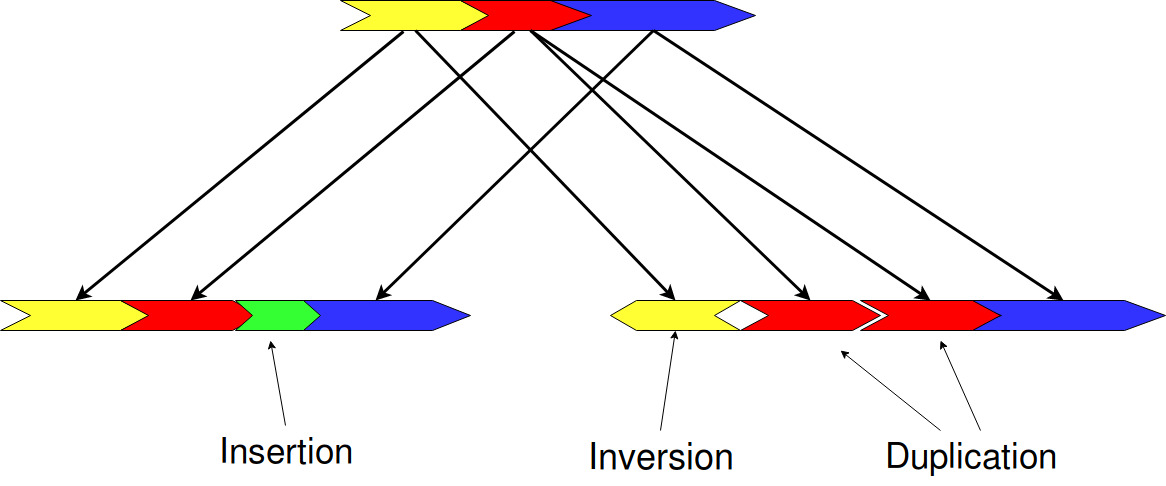
\includegraphics[width=\textwidth]{figures/genome_history}
  \caption{A genome history graph of two species and their most recent common ancestor, showing a duplication, inversion, and an insertion.}
  \label{fig:ghg}
\end{figure}

\begin{figure}[h]
  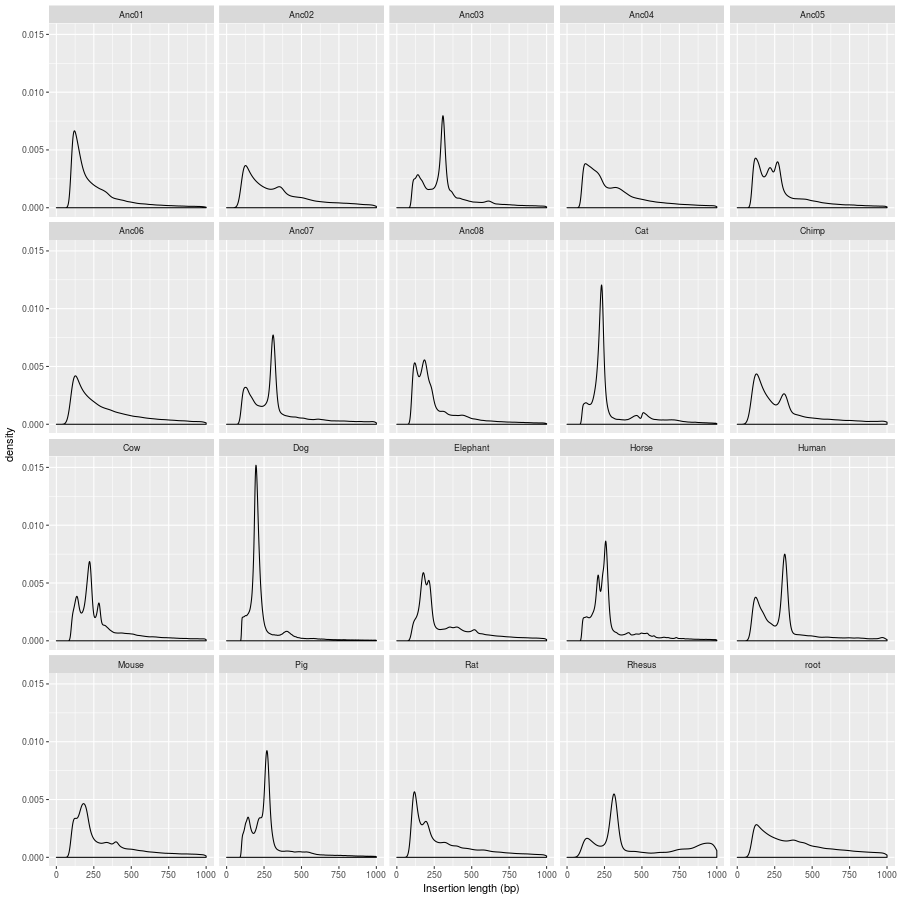
\includegraphics[width=\textwidth]{figures/insertion_lengths_normalized}
  \caption{Distribution of lengths of insertions along each branch in a 10-way Cactus alignment"}
  \label{fig:insertion_length_dist}
\end{figure}

\begin{figure}[h]
  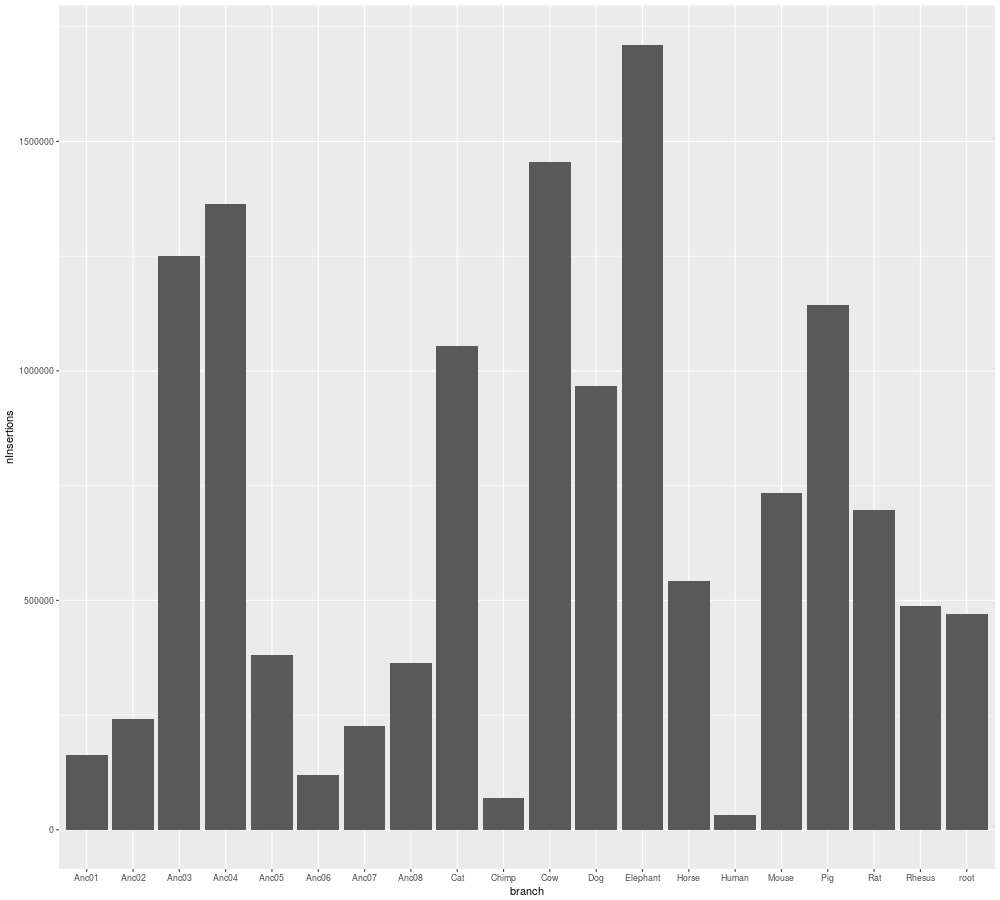
\includegraphics[width=\textwidth]{figures/nInsertionsPerBranch}
  \caption{Number of candidate insertions along each branch of a ten-way Cactus alignment}
  \label{fig:number_of_insertions}
\end{figure}

\section{Classifying Transposable Elements}

After candidate TE insertions have been extracted from a Cactus alignment, they can be clustered into families to produce TE annotations for each of the genomes. One way to do this is to create a multiple sequence alignment of all the candidate TEs, which could be represented as a forest of sequence graphs, with a graph representing each family. However, the candidate TEs should first be clustered into families using a more efficient kmer similarity method, to avoid performing sequence alignment on every pair of candidate TEs. A common measure of kmer similarity between two sequences is the Jaccard distance:
\begin{equation}
  d = \frac{|S_1 \cap S_2|}{|S_1 \cup S_2|},
\end{equation}
where $S_1$ and $S_2$ are the sets of kmers in the two sequences. The pairwise Jaccard distances between a set of sequences can be computed by taking advantage of sparsity, by first building an index mapping each kmer to the multiset of sequences that contain it, and then traversing the kmer index to fill in the pairwise Jaccard distances according to:
\begin{equation}
  d = \frac{|S_1 \cap S_2|}{|S_1| + |S_2| - |S_1 \cap S_2|}
\end{equation}
Sequences can then be joined into the same cluster if their Jaccard distance is above a certain threshold. To scale this method up to sets of millions of candidate TE insertions, such as in the Cow and Cat branches of the ten-way alignment, the set of candidate insertions can be broken into chunks and the above procedure performed on each chunk to yield (possibly redundant) clusters. The pairwise Jaccard distance can then be efficiently estimated between each pair of clusters by sampling kmers uniformly from all sequences in the cluster. Then highly similar clusters can be joined together.

Figure \ref{fig:after_selection} shows the normalized length distributions of the candidate insertions, compared to the insertions that were joined into families of size at least $5$ by the clustering procedure.

To evaluate the quality of the annotations produced by this method, they can be compared against the RepeatMasker database of known repetitive elements. One measure for the agreement between two sets of annotations is the Rand index:
\begin{equation}
  A = \{(i,j) \mid X_i = X_j, Y_i = Y_j\}
\end{equation}
\begin{equation}
  B = \{(i,j) \mid X_i \neq X_j, Y_i \neq Y_j\}
\end{equation}
\begin{equation}
  r = \frac{|A| + |B|}{\binom{n}{2}}
\end{equation}
where $X$ and $Y$ are the two annotations of the $n$ elements. Table \ref{tab:rmask_agreement} shows the agreement between the annotations produced with this method and the RepeatMasker database, as well as the coverage of the RepeatMasker annotations.

\begin{table}[H]
  \begin{center}
    \begin{tabular}{l|c|r}
      \text{Branch} & $r$ & \text{Fraction covered by RepeatMasker} \\
      \hline
      Human & 0.73 & 0.988 \\
      Mouse & -- & 0.960 \\
    \end{tabular}
    \caption{Agreement between RepeatMasker and annotations produced with this method}
    \label{tab:rmask_agreement}
  \end{center}
\end{table}

\begin{figure}[h]
  \begin{subfigure}[b]{0.5\textwidth}
    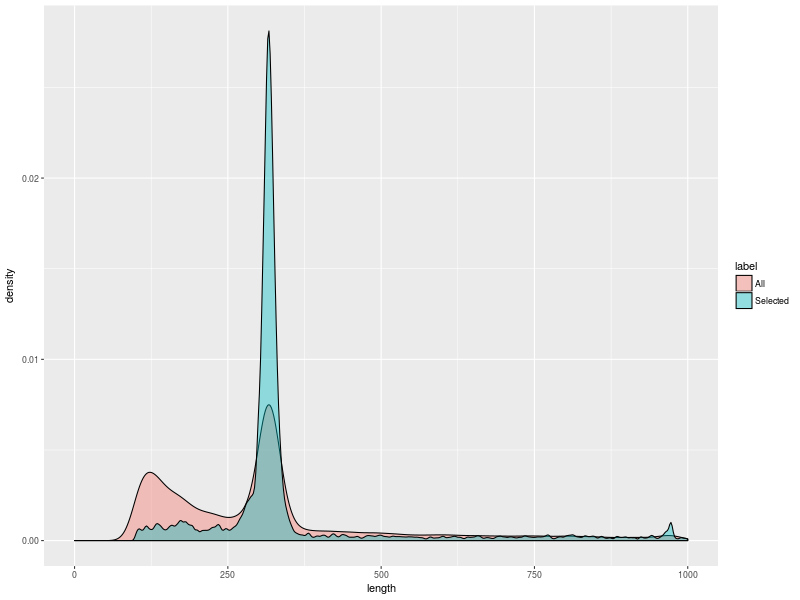
\includegraphics[width=\textwidth]{figures/human_clustered_dist}
    \caption{Human}
  \end{subfigure}
  \begin{subfigure}[b]{0.5\textwidth}
    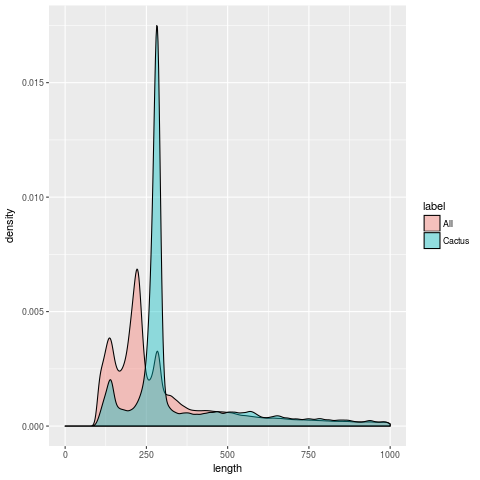
\includegraphics[width=\textwidth]{figures/cow_clustered_dist}
    \caption{Cow}
  \end{subfigure}
  \begin{subfigure}[b]{0.5\textwidth}
    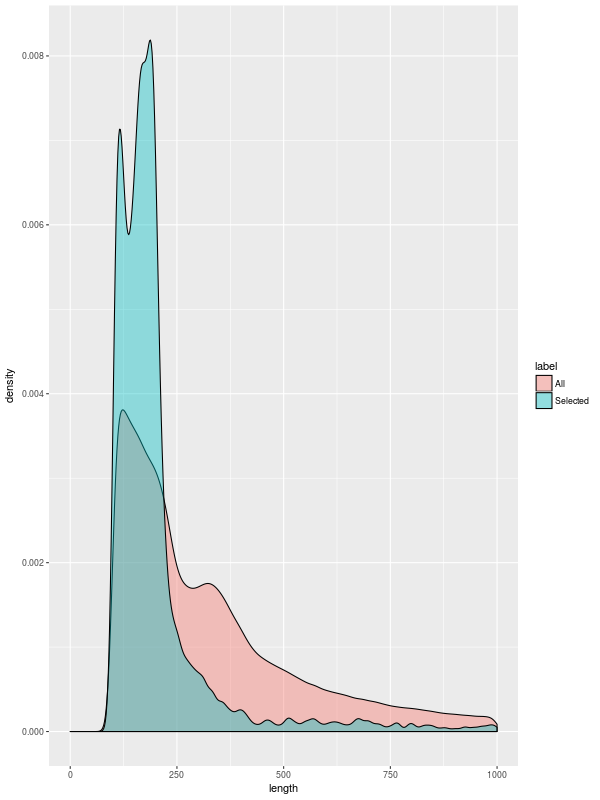
\includegraphics[width=\textwidth]{figures/anc04_clustered_dist}
    \caption{Mouse-Rat ancestor}
  \end{subfigure}
  \caption{Length distributions for the candidate TE insertions compared to the length distributions of the insertions that were found to be in clusters of at least 5.}
  \label{fig:after_selection}
\end{figure}


\end{document}
